% Created by tikzDevice version 0.6.2-92-0ad2792 on 2012-09-16 02:02:09
% !TEX encoding = UTF-8 Unicode
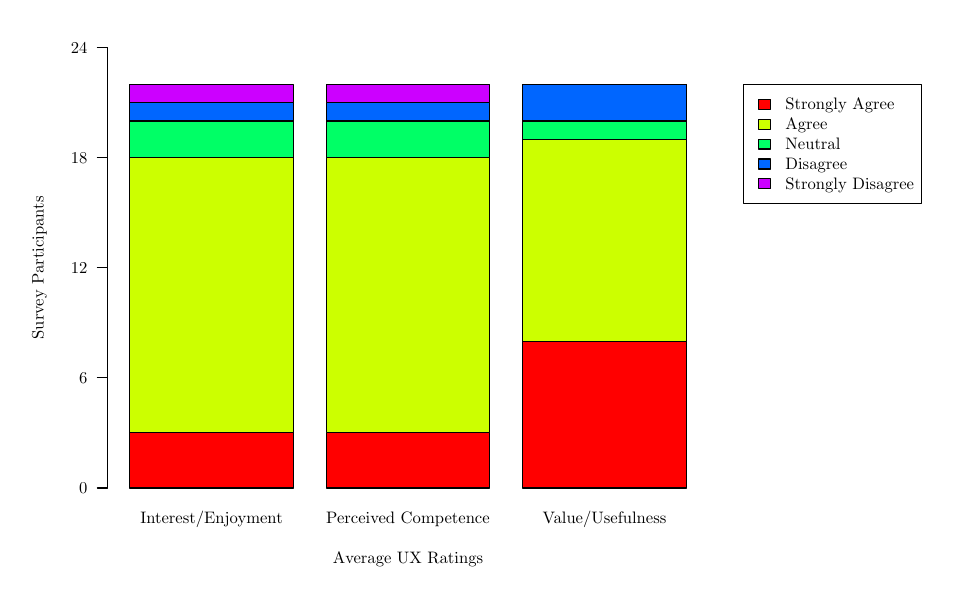
\begin{tikzpicture}[x=1pt,y=1pt]
\definecolor[named]{fillColor}{rgb}{1.00,1.00,1.00}
\path[use as bounding box,fill=fillColor,fill opacity=0.00] (0,0) rectangle (332.44,195.13);
\begin{scope}
\path[clip] (  0.00,  0.00) rectangle (332.44,195.13);
\definecolor[named]{drawColor}{rgb}{0.00,0.00,0.00}
\definecolor[named]{fillColor}{rgb}{1.00,0.00,0.00}

\path[draw=drawColor,line width= 0.4pt,line join=round,line cap=round,fill=fillColor] ( 36.85, 28.80) rectangle ( 96.01, 48.69);
\definecolor[named]{fillColor}{rgb}{0.80,1.00,0.00}

\path[draw=drawColor,line width= 0.4pt,line join=round,line cap=round,fill=fillColor] ( 36.85, 48.69) rectangle ( 96.01,148.15);
\definecolor[named]{fillColor}{rgb}{0.00,1.00,0.40}

\path[draw=drawColor,line width= 0.4pt,line join=round,line cap=round,fill=fillColor] ( 36.85,148.15) rectangle ( 96.01,161.41);
\definecolor[named]{fillColor}{rgb}{0.00,0.40,1.00}

\path[draw=drawColor,line width= 0.4pt,line join=round,line cap=round,fill=fillColor] ( 36.85,161.41) rectangle ( 96.01,168.04);
\definecolor[named]{fillColor}{rgb}{0.80,0.00,1.00}

\path[draw=drawColor,line width= 0.4pt,line join=round,line cap=round,fill=fillColor] ( 36.85,168.04) rectangle ( 96.01,174.67);
\definecolor[named]{fillColor}{rgb}{1.00,0.00,0.00}

\path[draw=drawColor,line width= 0.4pt,line join=round,line cap=round,fill=fillColor] (107.84, 28.80) rectangle (167.00, 48.69);
\definecolor[named]{fillColor}{rgb}{0.80,1.00,0.00}

\path[draw=drawColor,line width= 0.4pt,line join=round,line cap=round,fill=fillColor] (107.84, 48.69) rectangle (167.00,148.15);
\definecolor[named]{fillColor}{rgb}{0.00,1.00,0.40}

\path[draw=drawColor,line width= 0.4pt,line join=round,line cap=round,fill=fillColor] (107.84,148.15) rectangle (167.00,161.41);
\definecolor[named]{fillColor}{rgb}{0.00,0.40,1.00}

\path[draw=drawColor,line width= 0.4pt,line join=round,line cap=round,fill=fillColor] (107.84,161.41) rectangle (167.00,168.04);
\definecolor[named]{fillColor}{rgb}{0.80,0.00,1.00}

\path[draw=drawColor,line width= 0.4pt,line join=round,line cap=round,fill=fillColor] (107.84,168.04) rectangle (167.00,174.67);
\definecolor[named]{fillColor}{rgb}{1.00,0.00,0.00}

\path[draw=drawColor,line width= 0.4pt,line join=round,line cap=round,fill=fillColor] (178.83, 28.80) rectangle (238.00, 81.84);
\definecolor[named]{fillColor}{rgb}{0.80,1.00,0.00}

\path[draw=drawColor,line width= 0.4pt,line join=round,line cap=round,fill=fillColor] (178.83, 81.84) rectangle (238.00,154.78);
\definecolor[named]{fillColor}{rgb}{0.00,1.00,0.40}

\path[draw=drawColor,line width= 0.4pt,line join=round,line cap=round,fill=fillColor] (178.83,154.78) rectangle (238.00,161.41);
\definecolor[named]{fillColor}{rgb}{0.00,0.40,1.00}

\path[draw=drawColor,line width= 0.4pt,line join=round,line cap=round,fill=fillColor] (178.83,161.41) rectangle (238.00,174.67);
\definecolor[named]{fillColor}{rgb}{0.80,0.00,1.00}

\path[draw=drawColor,line width= 0.4pt,line join=round,line cap=round,fill=fillColor] (178.83,174.67) rectangle (238.00,174.67);
\end{scope}
\begin{scope}
\path[clip] (  0.00,  0.00) rectangle (332.44,195.13);
\definecolor[named]{drawColor}{rgb}{0.00,0.00,0.00}

\node[text=drawColor,anchor=base,inner sep=0pt, outer sep=0pt, scale=  0.60] at ( 66.43, 15.84) {Interest/Enjoyment};

\node[text=drawColor,anchor=base,inner sep=0pt, outer sep=0pt, scale=  0.60] at (137.42, 15.84) {Perceived Competence};

\node[text=drawColor,anchor=base,inner sep=0pt, outer sep=0pt, scale=  0.60] at (208.42, 15.84) {Value/Usefulness};
\end{scope}
\begin{scope}
\path[clip] (  0.00,  0.00) rectangle (332.44,195.13);
\definecolor[named]{drawColor}{rgb}{0.00,0.00,0.00}

\node[text=drawColor,anchor=base,inner sep=0pt, outer sep=0pt, scale=  0.60] at (137.42,  1.44) {Average UX Ratings};

\node[text=drawColor,rotate= 90.00,anchor=base,inner sep=0pt, outer sep=0pt, scale=  0.60] at (  5.76,108.36) {Survey Participants};
\end{scope}
\begin{scope}
\path[clip] (  0.00,  0.00) rectangle (332.44,195.13);
\definecolor[named]{drawColor}{rgb}{0.00,0.00,0.00}

\path[draw=drawColor,line width= 0.4pt,line join=round,line cap=round] ( 28.80, 28.80) -- ( 28.80,187.93);

\path[draw=drawColor,line width= 0.4pt,line join=round,line cap=round] ( 28.80, 28.80) -- ( 25.20, 28.80);

\path[draw=drawColor,line width= 0.4pt,line join=round,line cap=round] ( 28.80, 68.58) -- ( 25.20, 68.58);

\path[draw=drawColor,line width= 0.4pt,line join=round,line cap=round] ( 28.80,108.36) -- ( 25.20,108.36);

\path[draw=drawColor,line width= 0.4pt,line join=round,line cap=round] ( 28.80,148.15) -- ( 25.20,148.15);

\path[draw=drawColor,line width= 0.4pt,line join=round,line cap=round] ( 28.80,187.93) -- ( 25.20,187.93);

\node[text=drawColor,anchor=base east,inner sep=0pt, outer sep=0pt, scale=  0.60] at ( 21.60, 26.73) {0};

\node[text=drawColor,anchor=base east,inner sep=0pt, outer sep=0pt, scale=  0.60] at ( 21.60, 66.52) {6};

\node[text=drawColor,anchor=base east,inner sep=0pt, outer sep=0pt, scale=  0.60] at ( 21.60,106.30) {12};

\node[text=drawColor,anchor=base east,inner sep=0pt, outer sep=0pt, scale=  0.60] at ( 21.60,146.08) {18};

\node[text=drawColor,anchor=base east,inner sep=0pt, outer sep=0pt, scale=  0.60] at ( 21.60,185.86) {24};
\end{scope}
\begin{scope}
\path[clip] (  0.00,  0.00) rectangle (332.44,195.13);
\definecolor[named]{drawColor}{rgb}{0.00,0.00,0.00}

\path[draw=drawColor,line width= 0.4pt,line join=round,line cap=round] (258.70,174.67) rectangle (323.00,131.47);
\definecolor[named]{fillColor}{rgb}{1.00,0.00,0.00}

\path[draw=drawColor,line width= 0.4pt,line join=round,line cap=round,fill=fillColor] (264.10,169.27) rectangle (268.42,165.67);
\definecolor[named]{fillColor}{rgb}{0.80,1.00,0.00}

\path[draw=drawColor,line width= 0.4pt,line join=round,line cap=round,fill=fillColor] (264.10,162.07) rectangle (268.42,158.47);
\definecolor[named]{fillColor}{rgb}{0.00,1.00,0.40}

\path[draw=drawColor,line width= 0.4pt,line join=round,line cap=round,fill=fillColor] (264.10,154.87) rectangle (268.42,151.27);
\definecolor[named]{fillColor}{rgb}{0.00,0.40,1.00}

\path[draw=drawColor,line width= 0.4pt,line join=round,line cap=round,fill=fillColor] (264.10,147.67) rectangle (268.42,144.07);
\definecolor[named]{fillColor}{rgb}{0.80,0.00,1.00}

\path[draw=drawColor,line width= 0.4pt,line join=round,line cap=round,fill=fillColor] (264.10,140.47) rectangle (268.42,136.87);

\node[text=drawColor,anchor=base west,inner sep=0pt, outer sep=0pt, scale=  0.60] at (273.82,165.40) {Strongly Agree};

\node[text=drawColor,anchor=base west,inner sep=0pt, outer sep=0pt, scale=  0.60] at (273.82,158.20) {Agree};

\node[text=drawColor,anchor=base west,inner sep=0pt, outer sep=0pt, scale=  0.60] at (273.82,151.00) {Neutral};

\node[text=drawColor,anchor=base west,inner sep=0pt, outer sep=0pt, scale=  0.60] at (273.82,143.80) {Disagree};

\node[text=drawColor,anchor=base west,inner sep=0pt, outer sep=0pt, scale=  0.60] at (273.82,136.60) {Strongly Disagree};
\end{scope}
\end{tikzpicture}
